\documentclass[a4paper,11pt]{article}
\usepackage[polish]{babel}
\usepackage[MeX]{polski}
\usepackage[utf8]{inputenc} % latin2 lub cp1250
\usepackage[T1]{fontenc}
\usepackage{listings}
\usepackage{graphicx}
\usepackage{subfigure}



\title{Artykuł w Latexu}
\date{3 stycznia 2017}
\author{Imiona i nazwiska autorów}

\begin{document}
\maketitle{} %% obowiazkow po begin document
\pagenumbering{gobble}
\newpage{} %% po porstu tworzy nowa strone
\tableofcontents{}
\pagenumbering{arabic}



\section{\LaTeX\ w Wikipedii}
\LaTeX\ (od [Leslie] Lamport TeX) – oprogramowanie do zautomatyzowanego składu
tekstu, a także związany z nim język znaczników, służący do formatowania dokumentów
tekstowych i tekstowo-graficznych (na przykład: broszur, artykułów,
książek, plakatów, prezentacji, a nawet stron HTML) \cite{wikipedia_cytat}

LaTeX zajmuje się również odpowiednim rozmieszczeniem i sformatowaniem
wzorów matematycznych, rysunków i diagramów, zwalniając użytkownika ze
żmudnej pracy związanej z integracją tych elementów z właściwym tekstem.

W sposób automatyczny tworzone są:
\begin{itemize}
	\item spisy treści, ilustracji oraz tabel,
	\item numerowanie i referencje do rozdziałów i podrozdziałów,
	\item numerowanie i referencje obiektów takich jak wzory i rysunki,
	\item skorowidze,
	\item bibliografia.
\end{itemize}

\section{Wzory matematyczne w \LaTeX\/u}
\subsection{Ciągła transformata Fouriera}
Ciagłą transformatę Fouriera definiuje się następująco \cite{fourie}:

\begin{equation}
	\widehat{f}(\xi) = \mathcal{F}\{f(x)\} = \int\limits_{-\infty}^{\infty}f(x)e^{-2\pi x i \xi}
\end{equation}

gdzie zmienna niezalezna x reprezentuje czas, a zmienna transformaty $\xi$ reprezentuje częstotliwość.
 Pod pewnymi warunkami oryginał f może być odtworzony z transformaty $\widehat{f}$ 
przy pomocy transformaty odwrotnej \cite{fourie}:

\begin{equation}
	 f(x) = \mathcal{F}^{-1}\{\widehat{f}(\xi)\} = \int\limits_{-\infty}^{\infty}\widehat{f}(\xi)e^{-2\pi x i \xi}
\end{equation}

\subsection{Dyskretna transformata Fouriera}
Dyskretna Transformata Fouriera dana jest wzorem\cite{fourie2}:

\begin{equation}
	F_{DFT}(k) = \sum\limits_{n = 0}^{N - 1}f(n)e^{-j\displaystyle \frac{2\pi}{N} nk} dx
\end{equation}

gdzie n to indeks dyskretnego czasu, a k to indeks dyskretnych częstotliwości.
Transformata odwrotna zdefiniowana jest następująco\cite{fourie2}:

\begin{equation}
	f(n) = \frac{1}{N}\sum\limits_{k=0}^{N-1}F_{DFT}(k)e^{j\displaystyle \frac{2\pi}{N} nk} dx
\end{equation}


\subsection{Elementarne Macierze Rotacji}

Elementarne macierze transformacji to macierze opisujące zależność pomiędzy
współrzędnymi wskazanego punktu przed i po transformacji. Przez transformację
rozumiemy w tym przypadku rotację (czyli obrót). Np. obrót punktu wokół
osi $x$ o kat $\alpha$ opisany jest macierzą:

$$ RotX(\alpha) = \left [ \begin{array}{ccc}
	1 & 1 & 0 \\
	0 & \cos({\alpha}) & -\sin({\alpha}) \\
	0 & \sin({\alpha}) & \cos({\alpha}) 
\end{array}
\right ] $$


\section{Tabele, listingi, rysunki}
\subsection{Tabele}

Tabela 1 zawiera przykładowe wyniki dwóch sprawdzianów.


$$\begin{tabular}{|c|c|c|c|}
\multicolumn{4}{c}{Tablica 1: Przykładowa Tabela}\\
Lp. & nr indeksu & \multicolumn{2}{|c|}{kolokwium}\\
\hline
&&I&II\\
\hline
1&3245&4,0&5,0\\
2&42546&3,5&4,0\\
3&32546&2,0&3,0
\end{tabular}$$


\subsection{Listing.}
Poniżej pokazany jest listing jednego ze skryptów z poprzednich zajęć

\lstset{language = Matlab}
\begin{lstlisting}

A = 1;
Tokr = 1;
N = 3;
Ts = 0.01;

t = 0:Ts:N*Tokr−Ts;

x1 = [A*ones(1 , Tokr/(2*Ts)), 1*A*ones(1 , Tokr/(2*Ts))];

x = [];
for i = 1:N
    x=[x,x1];
end

plot(t,x);
hold on;

axis([0 N*Tokr+0.5*Tokr -1.5 1.5]);
grid on;
title('sinus, f=1 , 2 , 3[ Hz ]');
xlabel ('t');
ylabel ('x(t)');


\end{lstlisting}

\subsection{Rysunki.}
Rysunek 3.3 zawiera wykres uzyskany na poprzednich zajęciach obrócony w
płaszczyźnie kartki o: 0, 90 i 30 stopni. Wysokość górnych rysunków wynosi
3 cm a szerokość dolnego 6 cm.\newline

Plik ten przygotowano w oparciu o \cite{czworeczka} i \cite{piateczka}



\begin{thebibliography}{99}

\bibitem{wikipedia_cytat} Wikipedia o LATEX w portalu http://pl.wikipedia.org/wiki/LaTeX.




\bibitem{fourie}  Kaiser, Gerald A Friendly Guide to Wavelets, Birkhäuser ( 1994 ).

\bibitem{fourie2} Zieliński, Tomasz P. Cyfrowe przetwarzanie sygnałów, WKŁ, Warszawa (
2005 ).






\bibitem{czworeczka} Podstawy Technik Informatycznych - Wprowadzenie do LATEX- wykład dostepny
na https://webmail1.cie.put.poznan.pl/moodle/.


\begin{figure}
 \centering
  \subfigure[Pierwszy.]
	{
		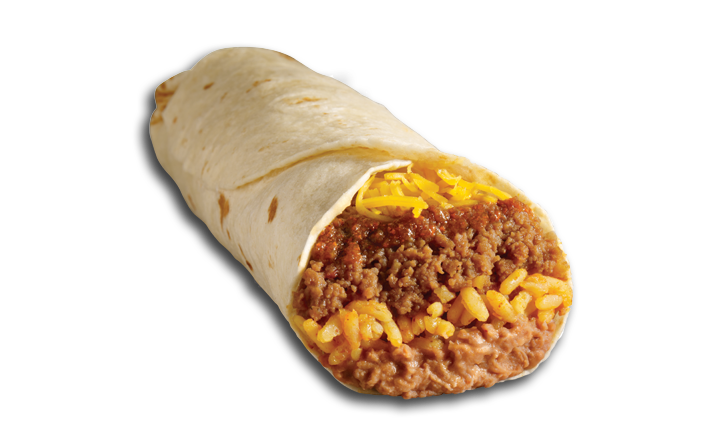
\includegraphics[angle=0,width = 0.30\textwidth, natwidth=700,natheight=400]{Images/Latex_picture_1.png}
	}
	\qquad
	\subfigure[Drugi.]
	{
		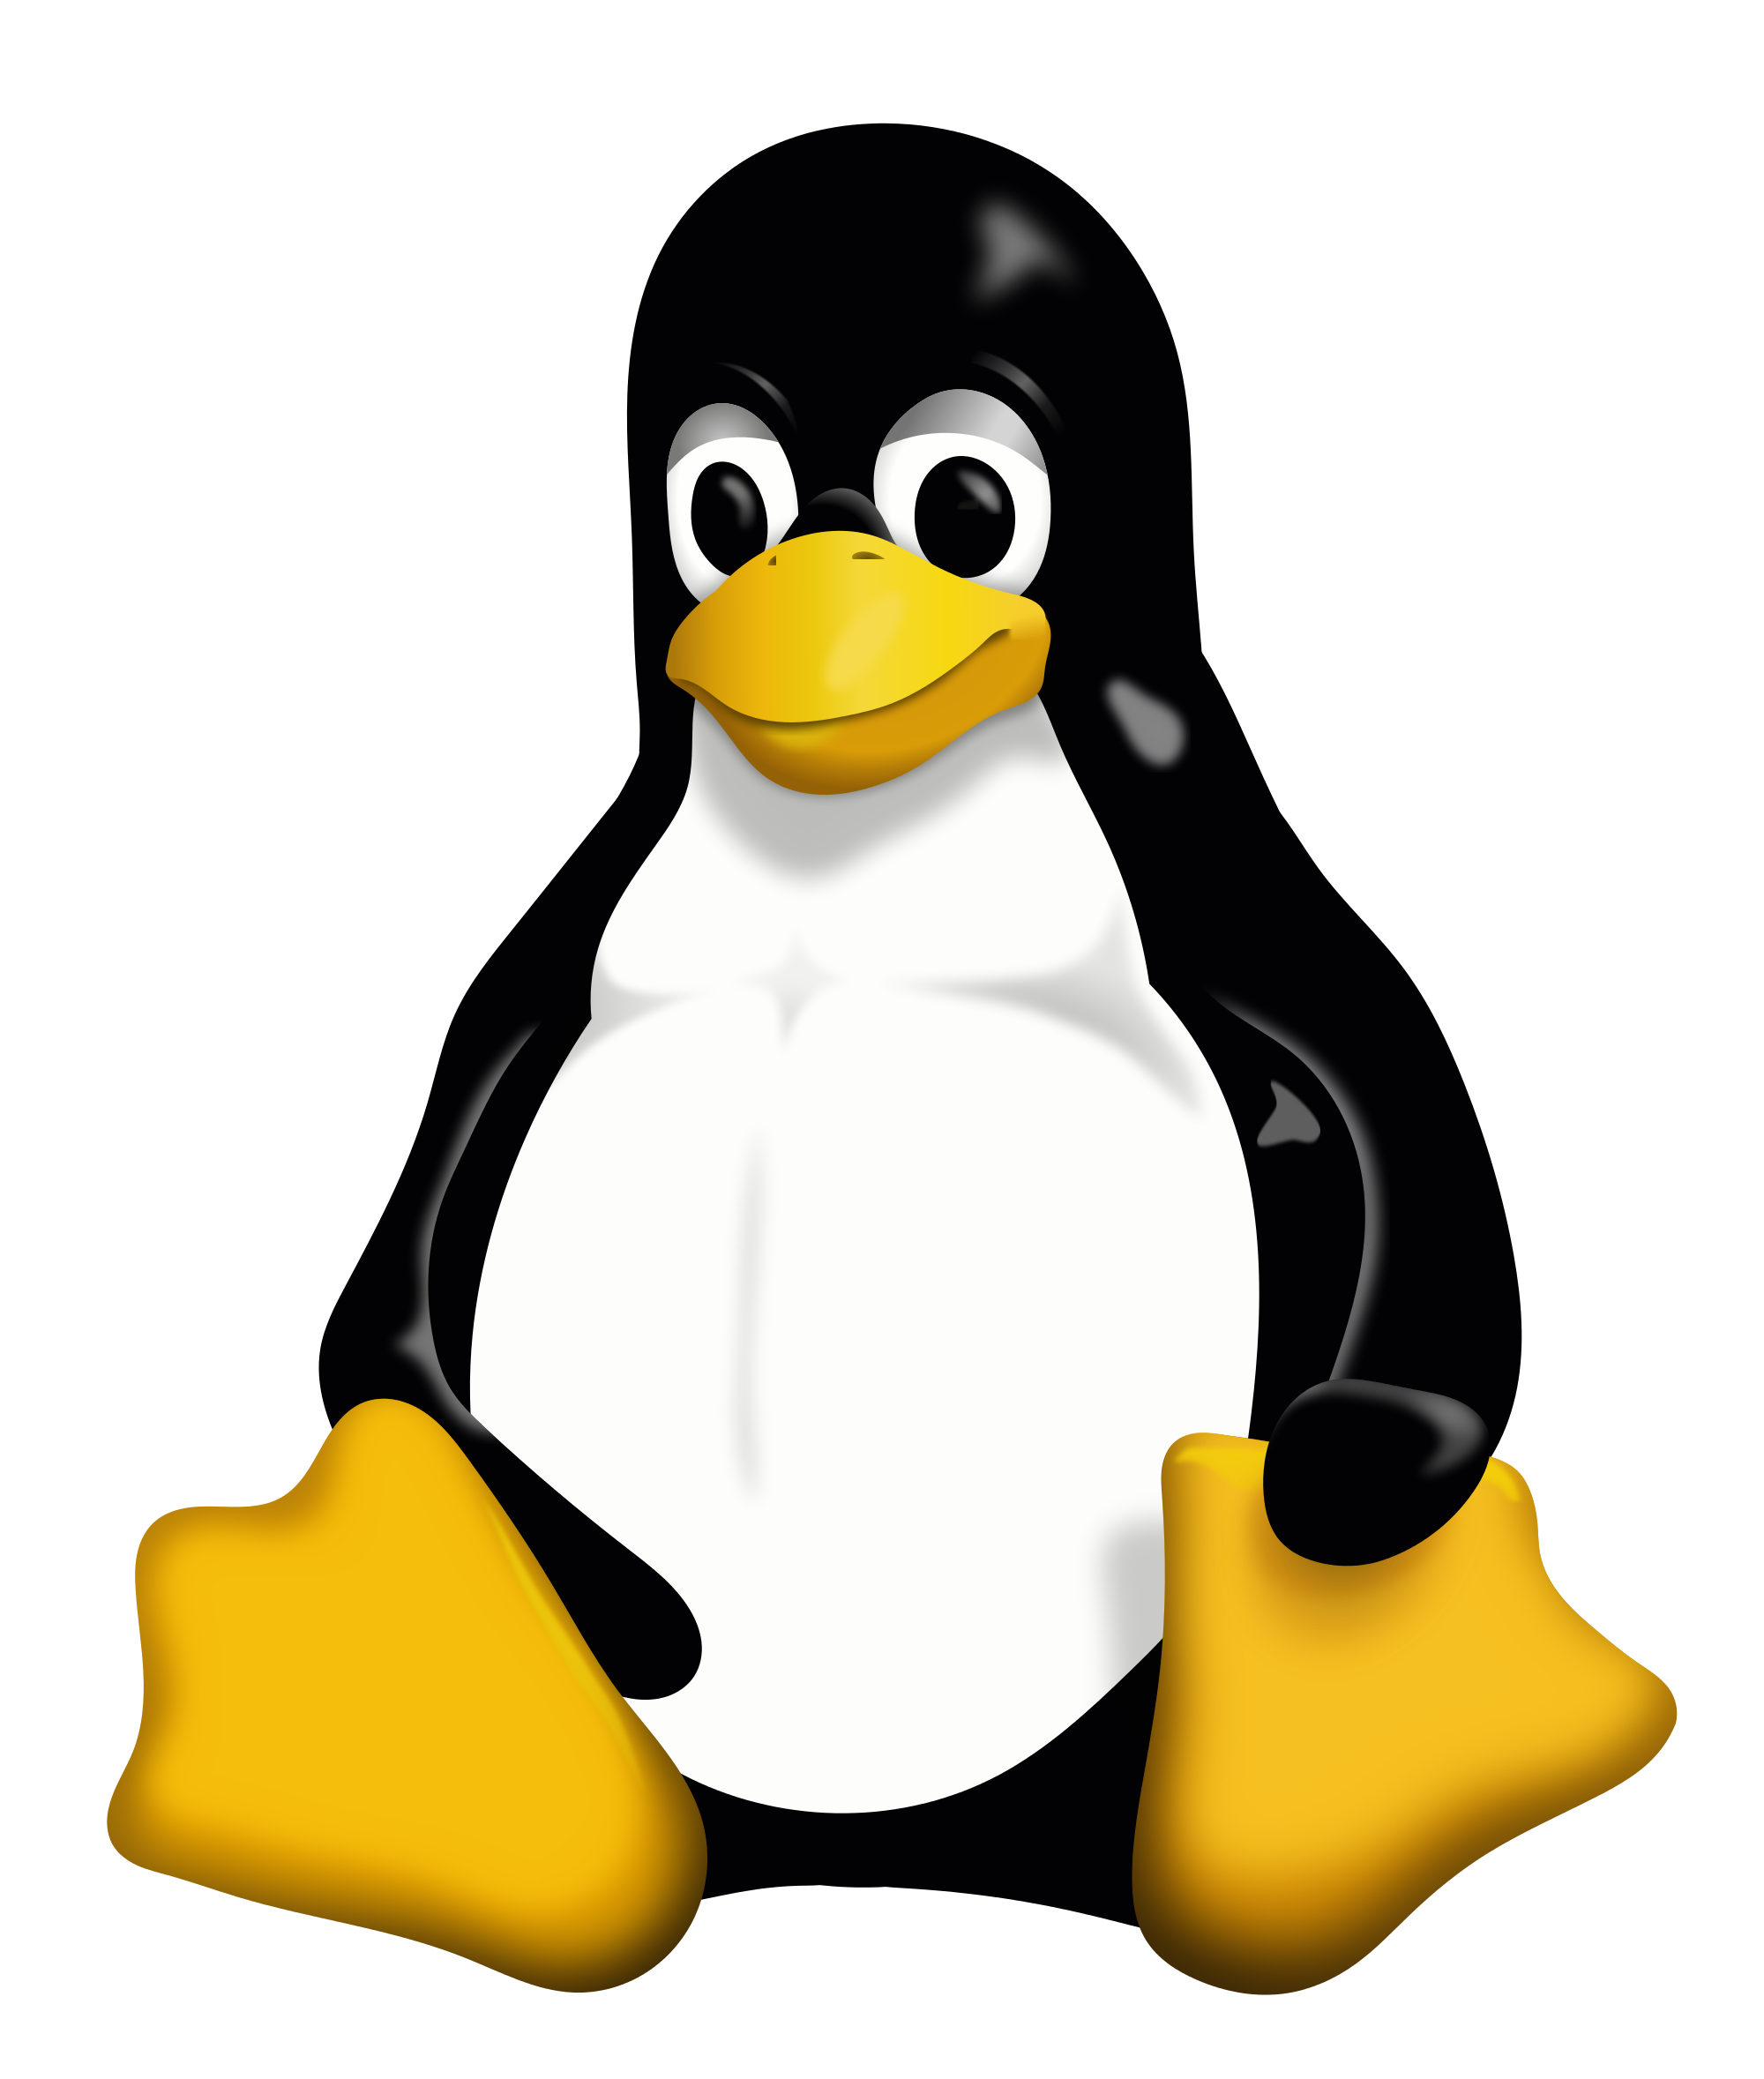
\includegraphics[angle=90,width = 0.10\textwidth, natwidth=400,natheight=400]{Images/Latex_picture_2.png}
	
	}
	\\
	\subfigure[Trzeci.]
	{
		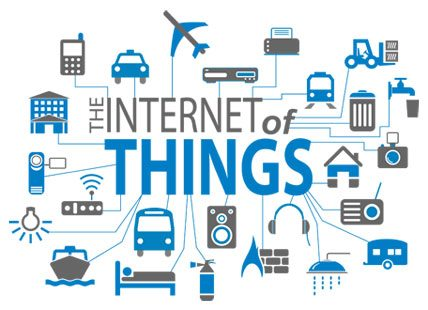
\includegraphics[angle=45,width = 0.5\textwidth, natwidth = 400, natheight = 400]{Images/Latex_picture_3.jpg}
	
	}
\end{figure}




\bibitem{piateczka} Helmut Kopka and PatrickW. Daly , A Guide to LATEX: Document Preparation
for Beginners and Advanced Users, fourth edition, Addison-Wes ley
( 2004 ).


\end{thebibliography}

\end{document}


